\section{Background of the Study}

With the fast growing technology and the capacity of computers are getting bigger, there comes the opportunity to create robots and new research in controlling them. These robots are mechanical, controlled by computers, and perform their work with precision. In robotics, one major component of a robot will be its core or the brain. These droids move on their own using the technology of artificial intelligence. Without humans behind them, they cannot perform complicated instructions \cite{Bharathi2013}. 

There are many ways to transfer data and control the mobile robot. Most use Bluetooth or wifi but these technologies fall short in coping up with the requirement of controlling sensors and control devices wirelessly. Zigbee has the fix for these control system. Zigbee is a technology based made for wireless communication. Some of its advantages are being low cost, low power consumption and low data rate \cite{Bharathi2013}. This alternative can make new opportunities for the mobile robot.

Android platform used for devices such as smartphones and tablets can be used as a control interface for robots and it provides sufficient resources and integrates more sensors. In android, java language can be used to program the interface and it is easier because of its modern software engineering. The challenge is that of connecting the control interface of android to the parts of the robot. 

\section{Problem Statement}

Nowadays many are having problems to go to certain locations due to harsh environment, life risking places etc. But still need to go due to certain conditions for example going for search and rescue during calamities. Many are trying to still do these but having their lives at risk as well is a very problematic problem. When a certain calamity arises in order to reach certain places many volunteers are needed or when you want to go to an expedition but you are not sure whether the terrain you are going to set foot on is safe you will need to have a volunteer to check the upcoming surrounding first. Especially when faced with natural calamities such as earthquake. With these in mind, robotic applications can be made in order to ease the tasks that are required also people can fully equip the robot with the technology needed to do certain tasks to ensure less risks and casualties.

By making use of a remote controlled robot people can avoid dangerous tasks or expeditions in areas that are hard to traverse.

\section{Objectives}
\subsection{General Objectives}
To design a remote controlled mobile robot for human search in inaccessible areas after an earthquake calamity
\subsection{Specific Objectives}
	
	\begin{itemize}
		\item	To create a mobile robot that carries a camera and has a connection with the use of ZigBee.
\item	To develop an algorithm that can manually control a mobile robot using a computer.
\item	To implement the algorithm for controlling the robot in Android.
\item	To design a land mobile robot for flat city terrain.
\item	To implement human detection with optical and auditory alarms.
\item	To achieve 70\% accuracy in detecting the human head.

	\end{itemize}
	
\section{Significance of the Study}

It has been difficult for people to take safety precautions when going to unknown lands. It has been very harsh especially when going to narrow places and dangerous places especially when there are natural calamities such as earthquakes and typhoons, people cannot reach or justify whether the place is safe to proceed or not. But autonomous robots have limitations especially when it comes to specifics like controlling the robots precisely. Manual control bypasses this problem by shifting the controls to the user and also allows for a more direct approach on tasks. Controlling the robot using android to explore dangerous terrain and searching for humans is what this proposal is about.

This proposal aims to build a rover for earthquake purposes that can be further enhanced for search and rescue operations or discovering unexplored territory. The rover can be navigated on dangerous places such as destroyed land and small or narrow places such as the aftereffects of earthquakes, you can use the rover to explore the terrain without the risk of getting killed by aftershocks or other unforeseen events. It can also detect whether there are humans or not in the unexplored areas.

This robotic project also incorporates the ZigBee communication protocol to control the Robotic module. ZigBee communication provides another dimension to Robotic control, mainly applied to manure the robot in remote areas, where the security of humans is risky. ZigBee communication utilizes the efficiency of RF communication and substitutes the Bluetooth communication, making the communication possible up to 1000\-1500 meters.

The robotic module may be effectively used to monitor a chaos situation using the wireless web cam mounted on the robot. The Robot is controlled by user friendly front end software developed in .NET. The project has a wide application in the security area. The module may be used to observe a hostage situation. The higher version of the robot may be used in areas where direct human approach is impossible.

\section{Scope and Delimitation}
\subsection{Scope and Delimitation}
\begin{itemize}
		\item	The mobile robot is designed to traverse flat solid terrain and not intended for steep inclines, sand/granulated ground, steps\stairs and severely uneven roads.
\item	The mobile robot would relay the camera's findings to the android interface in real-time
\item	The human detection system detects the human head, hand or torso.
\item	Implement a human detection system that would trigger an alarm on the android's screen and a beeping sound upon successful detection and achieve at least 70\% accuracy rate within 50 trial runs in various situations.
\end{itemize}
\subsection{Assumptions}
\begin{itemize}
	\item Battery life of the Android device may shorten due to the calculation load and the activated Bluetooth.
\end{itemize}

\section{Description and Methodology}
\subsection{Description}
\subsubsection{Mechanical}
Microcontroller PIC 16F877A the microcontroller acts like the brain of the wireless mobile robot system. The microcontroller chip that has been selected is PIC16F877A, manufactured by Microchip. The purpose of the IC among others is for controlling the speed of DC motor This chip is selected based on several reasons: first it is small in size and equipped with sufficient output ports without having to use a decoder or multiplexer. Second its portability and low current consumption. Third it has built\-in PWM which allow us to vary the duty cycle of DC motor drive. Fourth it is a very simple but powerful microcontroller. Users would only need to learn 35 single word instructions in order to program the chip. Fifth it can be programmed and reprogrammed easily (up to 10,000,000 cycles) using the universal programmer in robotics lab.
\subsubsection{Wireless Communication}
The vehicle would be controlled by a wireless remote controller. This wireless remote controller would control the movement of the vehicle. The remote controller that will be used in this project will be ZigBee based which uses Radio Frequency, Commercially available Remote Control (R\/C) units use small microcontrollers in the transmitter and receiver to send, receive and interpret data sent via radio frequency (RF). The receiver box has a PCB (printed circuit board) which comprises the receiving unit and a small servo motor controller. RF communication requires either a transmitter matched\/paired with a receiver, or a transceiver (which can both send and receive data). RF does not require line of sight and can also offer significant range (transmission distance). Standard radio frequency devices can allow for data transfer between devices as far away as several kilometers and there is seemingly no limit to the range for more professional RF units.
XBee and ZigBee modules use RF for communication, but allow the user to vary many of the communication parameters involved. These modules have a specific footprint (layout) and are only produced by certain companies. Their main advantage is that they provide a very robust easy to set up link and take care of all of the communication protocol details.
\subsubsection{Human Recognition}
The Human Recognition system will make use of a camera that will be interfaced through wireless communication to a computer that will have its own GUI (Graphical User Interface). The system will be able to detect Humans within the area based on a program that will allow the system to identify a person by comparing specific physical human attributes namely, the face, hand and torso, be it male or female.
We will make use of the implementation of the “Adaboost” algorithm and Haar\-like features, a common feature used for facial detection. The algorithm can be used specifically for training the database along with further applications on facial, hand and torso detection. 

\begin{figure}[h]
	\centering
		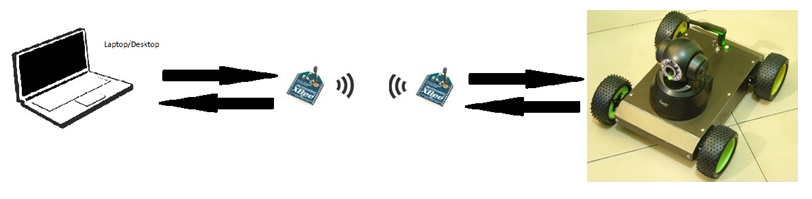
\includegraphics[width=5in]{model.png}
	\caption{System Model of the mobile robot}
	\label{fig:model}
\end{figure}

\subsection{Methodology}
\subsubsection{Electrical and Mechanical Testing}
In the mechanical design testing part, the prototype will be tested for its capability to traverse on land, the maximum speed that the system can attain when passing through different types of floor namely, Laminate, Stone, Tiles, Carpet, and Hardwood will be noted.

\subsubsection{Communication and Human Recognition Testing}
The system’s capability to be controlled by a wireless remote controller around areas with and without obstruction and its capability to detect humans in different positions will be tested. The first test will be conducted on rooms or certain areas within a city. The system must be able to detect a human face, hand or torso at a distance of at least 4 meters in daylight and 2 meters in dark areas. There will be 2\-3 different test subjects for every condition in this part of the experiment. The background of each test will be of white up to fairly decorated.
Next, the recognition system will be tested in a simulated environment. The number of frames transmitted per second will be determined by the timestamp that is part of the captured frames. Lastly, is the capability of the system to detect within a dark environment, the system has LED’s that can be turned ON when the surrounding is dark. This will help the system to see in dark areas.
The system’s capability to be controlled by an RC controller around areas with and without obstruction will be tested. The environment where the system will be tested will consist of different types of floors such as Laminate, Stone, Tiles, Carpet, and Hardwood. The first test will be conducted to see if the system can be controlled over a minimum distance of 200m line of sight without obstructions. A test whether the system can handle 200m line of sight will be conducted. The second test will involve controlling or traversing the vehicle over a distance with obstruction. We will characterize the maximum distance that the system can traverse when obstruction such as concrete and wooden walls are present, we will also obtain the maximum distance that the camera can still transmit video feed when there is obstruction such as wooden wall and concrete.

\section{Gantt chart}
\begin{figure}[h]
	\centering
		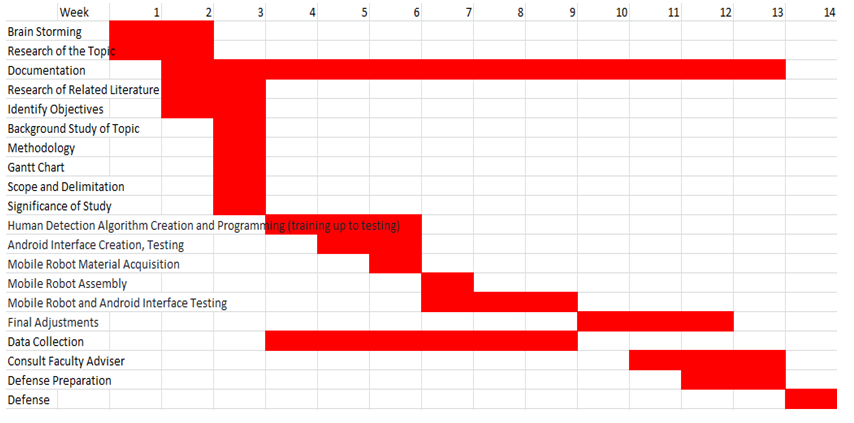
\includegraphics[width=5in]{gantt.png}
	\caption{Gantt chart}
	\label{fig:gantt}
\end{figure}
